% Result =================================================================================
\begin{frame}
	\section{Result and Discussion}
	\setbeamercolor{block title example}{use=structure,fg=white,bg=blue!80!black}
	\begin{beamercolorbox}[rounded=true]{block title example}
		\centering
		\LARGE
		Result and Discussion
	\end{beamercolorbox}
\end{frame}


%\begin{frame}
%	\frametitle{Result and Discussion}
%	\section{Result and Discussion}
%	\framesubtitle{Initialize Parameter}
%	\begin{columns}
%		\column{0.5\textwidth}
%		\begin{table}[h]
%			\begin{center}
%				\caption{Simulation Parameters}
%				\begin{tabular}{ccc}
%					Parameter                    &Value                            &Unit  \\
%					\hline
%					k1                           &5                                &-     \\
%					k2                           &10                               &-     \\
%					k3                           &10                               &-     \\
%					$r$                          &0.1                              &$m$   \\
%					$L$                          &0.2                              &$m$   \\
%					$Q$                          &$diag(1^2,0.52^2)\times 0.01$    &-     \\
%					$R$                          &$diag(1^2,1^2,1^2)\times 0.01$   &-     \\
%					%\hline
%					\hline
%				\end{tabular}
%			\end{center}
%		\end{table}
%		
%		
%		\column{0.5\textwidth}
%		\begin{table}[h]
%			\begin{center}
%				\caption{Sensor and Algorithm Data Publication Rate for EKF}
%				\begin{tabular}{ccc}
%					Data Publish                 &Rate             &Unit      \\
%					\hline
%					Encoder                      &20               &Hz        \\
%					IMU                          &10               &Hz        \\
%					Lidar Scan Match             &30               &Hz        \\
%					EKF Fusion                   &20               &Hz        \\
%					%\hline
%					\hline
%				\end{tabular}
%			\end{center}
%		\end{table}
%		
%		
%	\end{columns}
%\end{frame}




\begin{frame}
	\subsection{SLAM}
	\frametitle{Result and Discussion}
	\framesubtitle{SLAM}
	\begin{figure}
		%\caption{SLAM Result}
		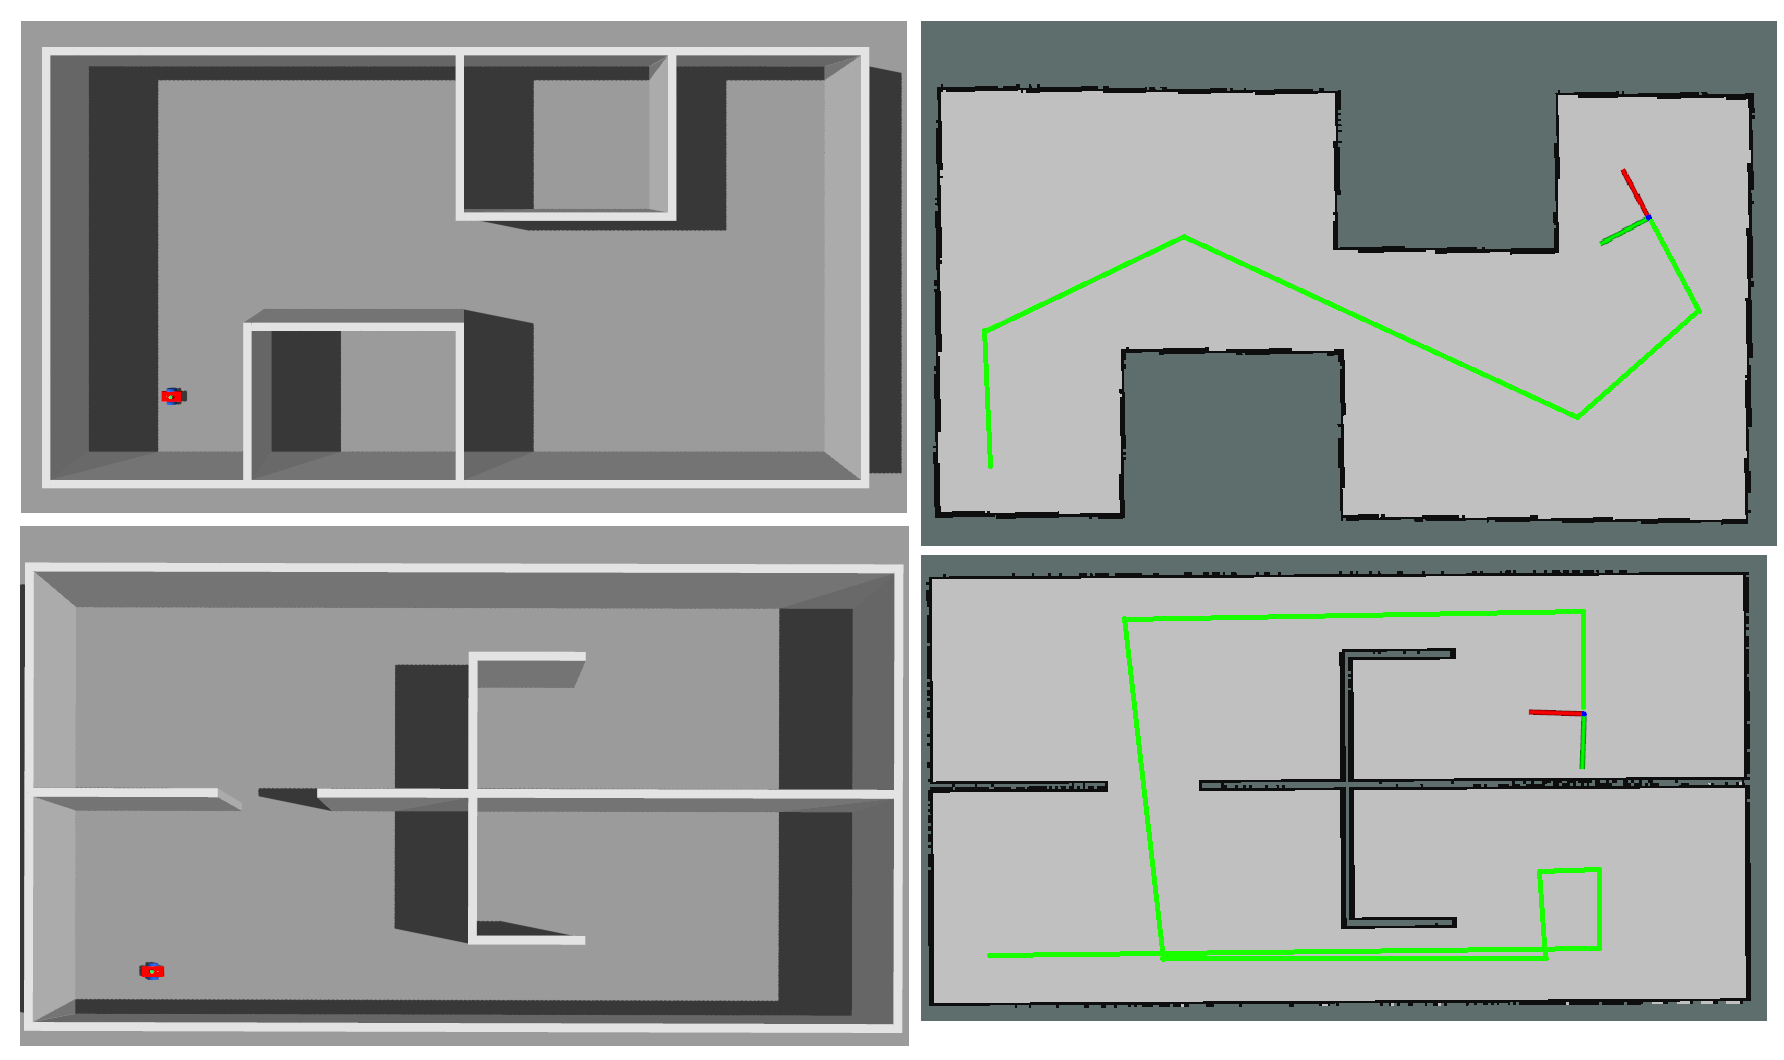
\includegraphics[scale=0.26]{image/slam_re}
	\end{figure}
\end{frame}


\begin{frame}
	\subsection{Path Planning}
	\frametitle{Result and Discussion}
	\framesubtitle{Path Planning}
	\begin{columns}
		\column{0.5\textwidth}
		\begin{figure}[h]
			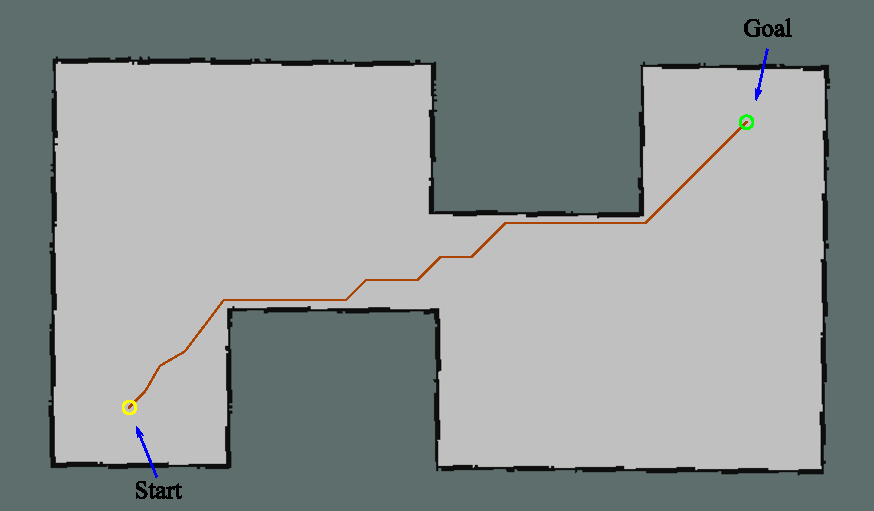
\includegraphics[scale=0.5]{image/pp_map1.pdf}
		\end{figure}
		
		\column{0.5\textwidth}
		\begin{figure}[h]
			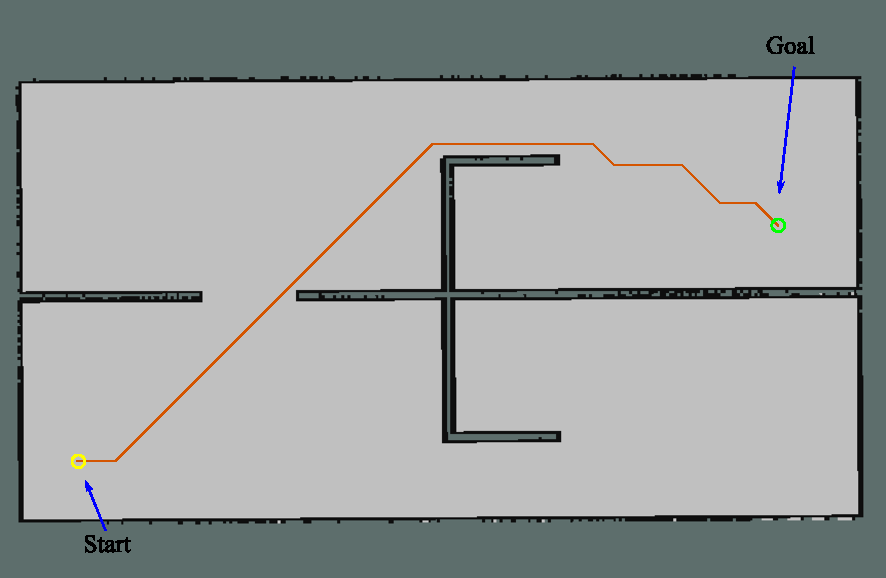
\includegraphics[scale=0.5]{image/pp_map2.pdf}
		\end{figure}
	\end{columns}
\end{frame}


\begin{frame}
	\subsection{Control}
	\frametitle{Result and Discussion}
	\framesubtitle{Control}
	\begin{columns}
		\column{0.5\textwidth}
		\begin{figure}[h]
			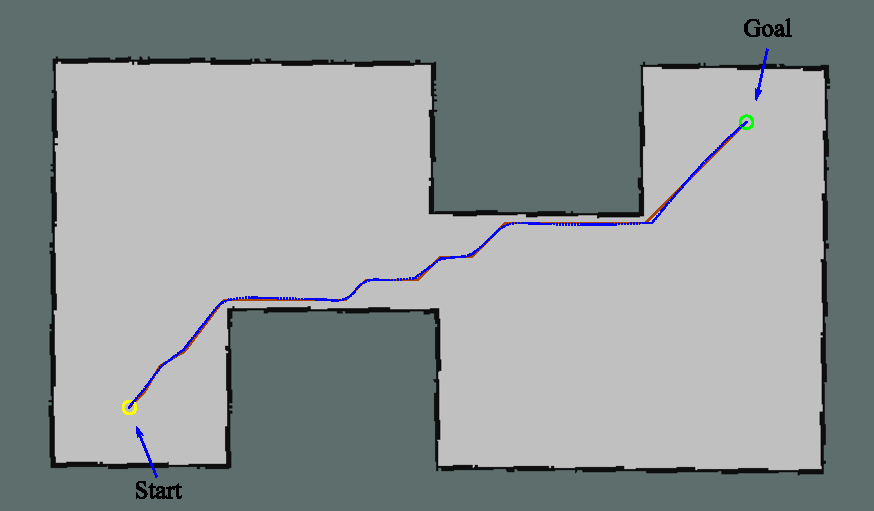
\includegraphics[scale=0.5]{image/ct_map1.pdf}
		\end{figure}
		
		\column{0.5\textwidth}
		\begin{figure}[h]
			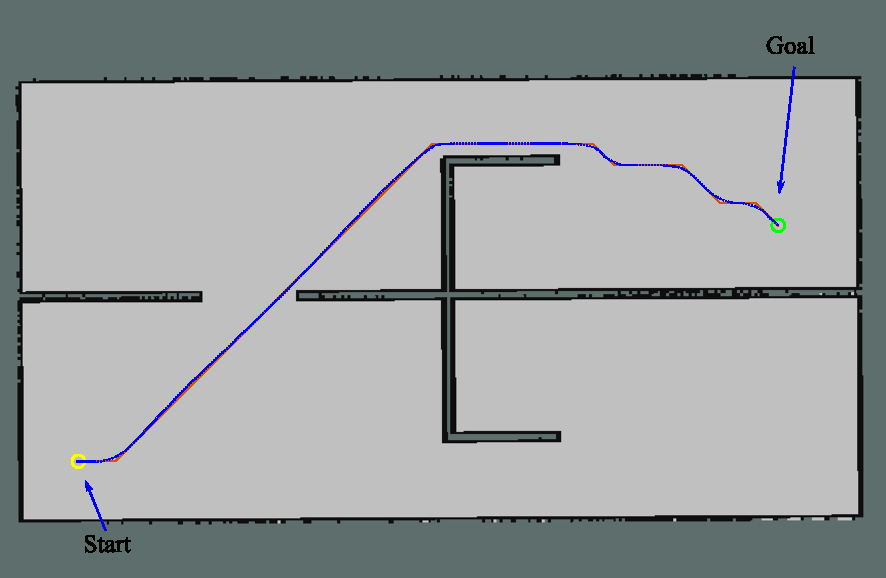
\includegraphics[scale=0.5]{image/ct_map2.pdf}
		\end{figure}
	\end{columns}
\end{frame}